\section{Resumo}
O subsistema de software está presente na interação máquina usuário englobando a gerência de pontuação pelo aplicativo, o reconhecimento do usuário e o reconhecimento e validação da garrafa. A integração será feita diretamente com o subsistema de eletrônica por meio da comunicação de requisições HTTP e indiretamente por meio de leituras de dados dos componentes eletrônicos, como a camêra frontal da máquina e o leitor de garrafa.

Para melhor descrição de alto nível do aplicativo, foi elaborado um documento de visão encontrado nos anexos, onde nele se encontram intervalos de qualidade, requisitos funcionais e diversos tópicos relevantes para sua elaboração.

A equipe de software também é responsável pela estrutura do banco de dados e pelo desenvolvimento da API que fará papel de interface de acesso ao BD, onde tanto o aplicativo quanto a Raspberry PI realizarão requisições.

\section{Prototipação}
Para a otimização do levantamento de Requisitos, foram realizadas reuniões com a equipe de eletrônica para poder nivelar os padrões e protocolos de comunicação entre os dois subsistemas. O protótipo inicial de comunicação ficou da seguinte forma:

\begin{figure}[!ht]
	\centering
		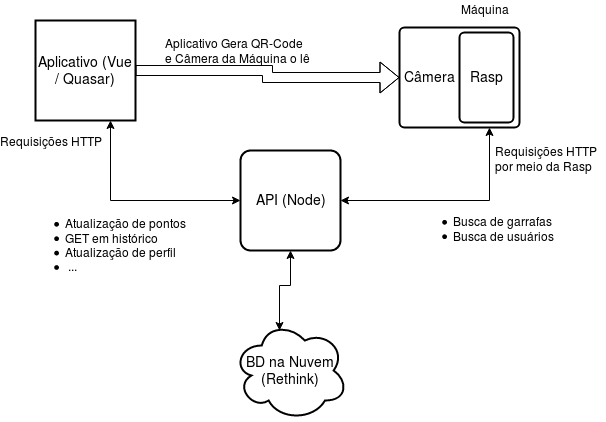
\includegraphics[scale=0.4]{figuras/software/1-prototipo-comunicacao.png}
	\caption{Protótipo de comunicação entre software e hardware.}
\end{figure}

Em relação aos requisitos do aplicativo, foram usados como suporte para levantamento e otimização, o documento de visão(em anexo), o diagrama de caso de uso e protótipos de alto nível (estes estão sendo utilizados nas descrições das funcionalidades no tópico seguinte).

\begin{figure}[!ht]
	\centering
		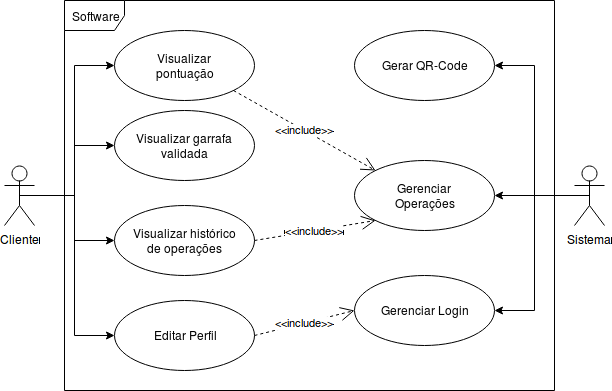
\includegraphics[scale=0.4]{figuras/software/2-Diagrama-de-Caso-de-Uso.png}
	\caption{Diagrama de Caso de Uso.}
\end{figure}

